\documentclass[aspectratio=169]{beamer}

\usepackage[T1]{fontenc}
\usepackage[utf8]{inputenc}
\usepackage{textcomp}
\usepackage{amsmath,amssymb}
\usepackage{booktabs}
\usepackage{array}
\usepackage{tikz}
\usetikzlibrary{positioning,arrows.meta}

\definecolor{aubburgundy}{RGB}{112,15,30}
\definecolor{aubburgundydark}{RGB}{80,10,22}
\definecolor{aubcharcoal}{RGB}{45,45,45}
\definecolor{aubgray}{RGB}{235,235,235}

\usetheme{default}
\usecolortheme{default}
\setbeamertemplate{navigation symbols}{}
\setbeamertemplate{footline}{}

\setbeamercolor{normal text}{fg=aubcharcoal,bg=white}
\setbeamercolor{structure}{fg=aubburgundy}
\setbeamercolor{itemize item}{fg=aubburgundy}
\setbeamercolor{itemize subitem}{fg=aubburgundydark}
\setbeamercolor{enumerate item}{fg=aubburgundy}
\setbeamercolor{bibliography item}{fg=aubburgundy}
\setbeamercolor{bibliography entry author}{fg=aubcharcoal}
\setbeamercolor{bibliography entry title}{fg=aubcharcoal}
\setbeamercolor{bibliography entry location}{fg=aubcharcoal}
\setbeamertemplate{itemize item}{\textcolor{aubburgundy}{\textbullet}}
\setbeamertemplate{itemize subitem}{\textcolor{aubburgundydark}{--}}

\tikzset{
  boxstyle/.style={rectangle, rounded corners, draw=aubburgundy, thick,
    fill=aubgray, minimum height=7mm, inner sep=4pt, align=center, font=\footnotesize},
  arrowstyle/.style={-{Latex[length=2mm]}, aubburgundy, thick}
}

\newcommand{\Dbar}{\bar D}
\newcommand{\Pbar}{\bar P}
\newcommand{\Bbar}{\bar B}

\begin{document}

% --- 1. formulation recap ---
\begin{frame}
\[
\max_{\pi}\ J_Q \qquad \text{s.t.} \qquad J_D\le\Dbar,\quad J_P\le\Pbar,\quad J_B\le\Bbar
\]
\[
J_j(\pi)=\sum_{t=0}^{35}\lambda^t c_j^t,\quad j\in\{D,P,B\},\quad \lambda=0.01
\]
\begin{itemize}
  \item $\Dbar=0.10,\ \Pbar=0.60,\ \Bbar=0.35$ -- calibrated experimentally, not assumed.
  \item Solved via Lagrangian relaxation on top of PPO, not a PPO built-in feature.
\end{itemize}
\note{Recap only -- this audience has seen the formulation before. Spend under a minute here.}
\end{frame}

% --- 2. lagrangian reward, multiplier update, why once per rollout ---
\begin{frame}
\[
r_{\mathrm L}^t=\beta_q\bar Q^t_{\text{viewport}}-\mu_D\frac{D^t}{T_0}-\mu_P\frac{P^t}{P_{\max}}-\mu_B\frac{\sum_i x_i^t}{N}
\]
\[
\mu_j \leftarrow \max\!\Bigl(0,\ \mu_j+\eta\bigl(\overline{J_j}^{\,\text{rollout}}-\bar b_j\bigr)\Bigr), \quad j\in\{D,P,B\}
\]
\begin{itemize}
  \item Multiplier updates once per rollout (2{,}048 steps); PPO does 320 gradient updates per rollout in between (10 epochs $\times$ 32 minibatches).
  \item \emph{``Convergence proofs have relied upon updating the multiplier more slowly than the policy parameters''} \cite{stooke20}, Related Work, citing \cite{tessler18}.
\end{itemize}
\note{This is the key defended design choice. Quote the Related Work sentence directly, page 2 of Stooke et al. -- have the PDF open and ready to show that paragraph.}
\end{frame}

% --- 3. Stooke et al. -- exact relevant content and correction ---
\begin{frame}
\begin{itemize}
  \item $J_C(\pi)=\mathbb{E}_{\tau\sim\pi}\bigl[\sum_{t=0}^{\infty}\gamma^t C(\cdot)\bigr]$ -- true value is an infinite-horizon expectation \cite{stooke20}, Sec.~3, Eq.~5.
  \item Algorithm 1 drives the multiplier with a \emph{sample estimate} $\hat J_C$, not the true $J_C$ -- same role as our $\overline{J_j}^{\text{rollout}}$.
  \item CPPO experiments: \emph{``the environments' finite horizons allowed use of non-discounted episodic costs as the constraint''} \cite{stooke20}, Sec.~6.2 -- same simplification we made (finite Monte Carlo return, no cost critic).
\end{itemize}
\vspace{6pt}
\footnotesize\textbf{Correction:} Algorithm 1's minibatch and $\lambda$ update happen together -- a \emph{tighter} coupling than ours, not looser. The slower-multiplier defense is the Related Work citation on the previous slide, not the minibatch structure itself.
\note{Show Algorithm 1 (page 5) live -- point at the 'sample estimate J-hat-C' line. Then show Section 6.2 (page 7) for the non-discounted episodic cost line. State the correction plainly: don't claim minibatch=rollout, that's not what supports us.}
\end{frame}

% --- 3b. how we satisfy the constraint: expectation, Monte Carlo, update ---
\begin{frame}
\footnotesize
True constraint (expectation over $\pi$'s trajectory distribution; $D$ shown, $P,B$ identical):
\[
\max_\pi\ \mathbb{E}_\pi[J_Q] \quad \text{s.t.} \quad \mathbb{E}_\pi[J_D]\le\Dbar, \qquad J_D=\sum_{t=0}^{35}\lambda^t\frac{D^t}{T_0}
\]
Same structure as \cite{stooke20}, Sec.~3, Eq.~5: $J_C(\pi)=\mathbb{E}_{\tau\sim\pi}\bigl[\sum_{t=0}^{\infty}\gamma^t C(\cdot)\bigr]$ -- an expectation over trajectories, not computable exactly without infinite sampling, in either setting.

\vspace{6pt}
\begin{center}
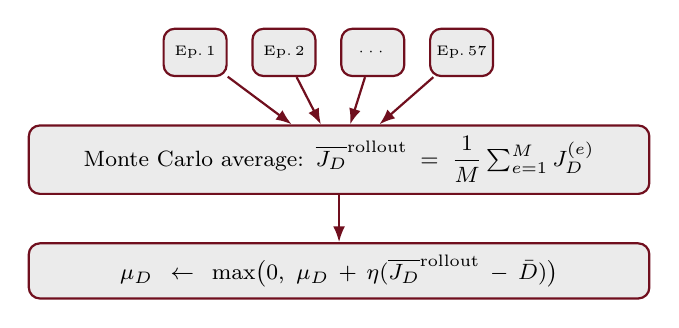
\begin{tikzpicture}[node distance=5mm]
  \tikzset{ep/.style={rectangle, rounded corners, draw=aubburgundy, thick,
    fill=aubgray, minimum height=6mm, minimum width=8mm, inner sep=2pt, align=center, font=\tiny}}
  \tikzset{big/.style={rectangle, rounded corners, draw=aubburgundy, thick,
    fill=aubgray, minimum height=7mm, inner sep=4pt, align=center, font=\footnotesize, text width=7.6cm}}
  \node[ep] (e1) {Ep.\,1};
  \node[ep, right=3mm of e1] (e2) {Ep.\,2};
  \node[ep, right=3mm of e2] (e3) {$\cdots$};
  \node[ep, right=3mm of e3] (e57) {Ep.\,57};
  \node[big, below=6mm of e2, xshift=7mm] (avg)
    {Monte Carlo average: $\overline{J_D}^{\text{rollout}}=\dfrac{1}{M}\sum_{e=1}^{M}J_D^{(e)}$};
  \node[big, below=6mm of avg] (upd)
    {$\mu_D\leftarrow\max\bigl(0,\ \mu_D+\eta(\overline{J_D}^{\text{rollout}}-\Dbar)\bigr)$};
  \draw[arrowstyle] (e1) -- (avg);
  \draw[arrowstyle] (e2) -- (avg);
  \draw[arrowstyle] (e3) -- (avg);
  \draw[arrowstyle] (e57) -- (avg);
  \draw[arrowstyle] (avg) -- (upd);
\end{tikzpicture}
\end{center}

\vspace{4pt}
$M\approx56$--$57$ episodes per rollout, each 36 steps -- same role as \cite{stooke20} Algorithm 1's sample estimate $\hat J_C$, drawn from ``sample a minibatch.'' Constraint is satisfied in expectation, not per step or per episode.
\note{Walk top to bottom: state the true (uncomputable) constraint first, cite Stooke Eq. 5 to show it's the same structure they use, then the diagram -- each box is one completed 36-step episode within the current rollout, all $\approx$57 of them get averaged into a single number, and that number is what actually moves $\mu_D$. Say explicitly: this average is our stand-in for the expectation, not the true expectation itself.}
\end{frame}

% --- 4. lambda=0.01 consequences ---
\begin{frame}
\[
\lambda=0.01 \ \Rightarrow\ \text{weights } 1,\ 0.01,\ 0.0001,\ldots
\]
\begin{itemize}
  \item Steps 2--35 contribute $<0.01\%$ -- $J_Q,J_D,J_P,J_B$ are effectively first-step statistics.
  \item PPO's own $\gamma=0.99\ne\lambda=0.01$ -- PPO's gradient targets $\sum_t 0.99^t r_{\mathrm L}^t$, not the $\lambda=0.01$-discounted Lagrangian.
  \item RCPO permits a mismatched ``guiding'' discount only under $\Theta_\gamma\subseteq\Theta$ \cite{tessler18} -- not verified here, difficult to demonstrate in this environment.
  \item Current implementation: approximate, not exact, solver of the stated equations.
\end{itemize}
\note{Two separate consequences of the same lambda choice -- make sure that distinction lands. The Theta-gamma subset condition is in RCPO's Theorem 2; mention it's the condition under which the mismatch would still be theoretically sound, and we can't currently show it holds.}
\end{frame}

% --- 5. rollout/episode boundary misalignment ---
\begin{frame}
\[
\gcd(2048,36)=4 \ \Rightarrow\ \text{9-rollout cycle: } 56,\,57,\,57,\,57,\,57,\,57,\,57,\,57,\,57,\ \ldots
\]
\begin{itemize}
  \item Verified against all 342 real rollouts of the 700K run -- zero mismatches with this predicted pattern.
  \item $\approx$89\% of rollouts contain one episode that began under the \emph{previous} rollout's policy.
  \item Effect: $\approx$1 of 56--57 episodes per multiplier update ($\approx$1.7\%) is not a clean single-policy sample.
\end{itemize}
\note{This one is fully our own finding, verified directly against the log -- not from either paper. Small effect, but real and precisely quantified, not just guessed at.}
\end{frame}

% --- 6. training setup recap ---
\begin{frame}
\begin{itemize}
  \item Runner video, 12 traces: 9 training / 3 validation (fixed, repeated every checkpoint).
  \item Observation $\omega^t=[Z^t,\Delta_\theta^{t-1},\Delta_\phi^{t-1},h^t]$, normalized online (VecNormalize), frozen at validation.
  \item Validated every rollout on the 3 fixed traces, fixed seeds; feasibility-first checkpoint selection.
\end{itemize}
\note{Brief context-setter before the results, in case it has been a while since the last meeting. Do not linger.}
\end{frame}

% --- 7. results progression ---
\begin{frame}
\begin{center}
{\scriptsize
\setlength{\tabcolsep}{4pt}
\begin{tabular}{lccc}
\toprule
Validation & $\approx$51.2K & $\approx$301K & 700{,}416 (final) \\
\midrule
Feasible & 0 & 0 & \textbf{1} \\
$J_D$ ($\le0.10$) & 0.2755 & 0.1379 & 0.0000 \\
$J_P$ ($\le0.60$) & 0.2525 & 0.2525 & 0.2525 \\
$J_B$ ($\le0.35$) & 0.4840 & 0.4051 & 0.1898 \\
Coverage & 0.904 & 0.858 & 0.840 \\
Stall (s) & 0.391 & 0.169 & 0.001 \\
Enh. tiles & 35.7 & 25.0 & 17.0 \\
\bottomrule
\end{tabular}}
\end{center}
\vspace{6pt}
\footnotesize 342 rollouts, 140/342 feasible, last 20/20 feasible.
\note{Headline result slide. 700K is the only run that reaches sustained feasibility.}
\end{frame}

% --- 8. results trade-offs ---
\begin{frame}
\begin{center}
{\footnotesize
\begin{tabular}{lcc}
\toprule
 & Start & End \\
\midrule
Coverage & 0.927 & 0.882 \\
Stall (s) & 0.531 & 0.022 \\
Power (mW) & 49.6 & 27.6 \\
Enh. tiles & 39.1 & 19.0 \\
\addlinespace
$\mu_D$ & 1.00 & 1.71 \\
$\mu_B$ & 1.00 & 1.46 \\
$\mu_P$ & 1.00 & 0.009 \\
\bottomrule
\end{tabular}}
\end{center}
\note{Real trade-off, not noise: coverage down 4.9 percent, everything else down sharply. mu_P collapsing to near zero means the power constraint is slack at the current budget.}
\end{frame}

% --- 9. issues summary ---
\begin{frame}
\begin{center}
{\scriptsize
\begin{tabular}{lc}
\toprule
Issue & Status \\
\midrule
$\gamma_{\text{PPO}}\ne\lambda$ (approximate solver) & Deferred \\
Rollout/episode misalignment ($\approx$1.7\% mixed) & Deferred \\
Single, non-parallelized environment & Not tried \\
Most PPO hyperparameters at library defaults & Not validated \\
Constant (not decreasing) multiplier learning rate & Known theory gap \\
VecNormalize vs.\ fixed constants & Not compared \\
Power constraint slack ($\mu_P\to0.009$) & Open question \\
\bottomrule
\end{tabular}}
\end{center}
\vspace{4pt}
\footnotesize Full list with root causes: \texttt{implementation\_review\_and\_ppo\_questions.md}.
\note{Don't read every row -- name two or three, then point to the document for the rest.}
\end{frame}

% --- 10. trade-offs behind modeling choices ---
\begin{frame}
\begin{itemize}
  \item $\gamma_{\text{PPO}}=0.99$ vs.\ $\lambda=0.01$: matching them would make PPO's own value estimation almost fully myopic; keeping them apart breaks exactness.
  \item Monte Carlo returns vs.\ a learned cost-critic: simpler, exact per episode, but only viable because episodes are short and always complete.
  \item VecNormalize (adaptive) vs.\ fixed constants: avoids needing pre-existing data, but introduces its own epsilon/variance issue.
  \item Lagrangian relaxation vs.\ CPO \cite{achiam17} / Lyapunov methods \cite{chow18}: tolerates violations during training (fine in simulation) in exchange for much lower implementation complexity.
\end{itemize}
\note{Each bullet is a real either/or, not a mistake. Keep this fast -- one line each.}
\end{frame}

% --- 11. PPO vs PPO+PDS+VE comparison plan ---
\begin{frame}
\begin{itemize}
  \item Primary: feasibility rate, $J_Q$ among feasible checkpoints, validation coverage/stall/power/tiles.
  \item Learning efficiency: steps to first/sustained feasibility, quality-vs-steps curve.
  \item Fairness: same budgets, same environment, same real-interaction count as the primary comparison; report wall-clock time and update count \emph{separately} (virtual experience adds updates, not real interactions).
  \item Never compare checkpoints by mean Lagrangian reward alone -- $\mu$'s shift during training.
\end{itemize}
\note{This is the plan, not a result -- no claim yet that PDS+VE is better. State that explicitly.}
\end{frame}

% --- 12. references ---
\begin{frame}
\footnotesize
\begin{thebibliography}{9}
\bibitem{altman99} E. Altman. \emph{Constrained Markov Decision Processes}. CRC Press, 1999.
\bibitem{tessler18} C. Tessler, D. J. Mankowitz, S. Mannor. Reward Constrained Policy Optimization. \emph{arXiv:1805.11074}, 2018 (ICLR 2019).
\bibitem{stooke20} A. Stooke, J. Achiam, P. Abbeel. Responsive Safety in Reinforcement Learning by PID Lagrangian Methods. \emph{ICML}, PMLR 119, 2020.
\bibitem{achiam17} J. Achiam, D. Held, A. Tamar, P. Abbeel. Constrained Policy Optimization. \emph{ICML}, 2017.
\bibitem{chow18} Y. Chow, O. Nachum, E. Du\'e\~nez-Guzm\'an, M. Ghavamzadeh. A Lyapunov-based Approach to Safe Reinforcement Learning. \emph{NeurIPS}, 2018.
\bibitem{chakareski25} J. Chakareski, L. Wang, N. Mastronarde. Reinforcement Learning-Based Dynamic Resource Allocation for Aerial 360\textdegree{} Video VR Streaming. \emph{MMSP}, 2025.
\end{thebibliography}
\note{Move through quickly, this is a reference slide.}
\end{frame}

% --- 13. questions ---
\begin{frame}
\begin{itemize}
  \item Keep $\lambda=0.01$, or change it -- and reconcile with $\gamma_{\text{PPO}}$?
  \item How many more steps to train?
  \item Are these the right evaluation metrics?
  \item Move next to comparing PPO vs.\ PPO + PDS + VE now?
  \item Tighten $\Pbar$, or narrow the power action range?
  \item Anything else from the issues list to prioritize first?
\end{itemize}
\note{Final slide. Some of these will already have come up earlier -- that is fine, restate them here as the concrete decision points to leave the meeting with.}
\end{frame}

\end{document}
